\documentclass[11pt]{article}
\usepackage{fullpage}
\usepackage{amsmath,amsthm,amssymb,amsfonts,multirow}
\usepackage{mathtools}
\usepackage{graphicx}
\usepackage{xcolor}
\usepackage{float}
%\usepackage{enumerate}
\usepackage[shortlabels, inline]{enumitem}
\usepackage{textcomp}
\usepackage{hyperref}
\usepackage{comment}

\usepackage{listings}
\lstset{language=Python, numbers=left, basicstyle=\ttfamily, keywordstyle=\color{blue}, showstringspaces=false}

\usepackage[style=alphabetic-verb]{biblatex}
% \bibliography{Problems/ref.bib}

\newcommand{\N}{\mathbb{N}}
\newcommand{\Z}{\mathbb{Z}}
\newcommand{\Q}{\mathbb{Q}}
\newcommand{\R}{\mathbb{R}}
\newcommand{\C}{\mathcal{C}}
\newcommand{\K}{\mathbb{K}}
\renewcommand{\div}{\mid}
\newcommand{\ndiv}{\nmid}
\newcommand{\E}{\mathbb{E}}
\newcommand{\I}{\mathbb{I}}
\newcommand{\F}{\mathcal{F}}

\DeclareMathOperator{\id}{Id}
\DeclareMathOperator{\tr}{Tr}
\DeclareMathOperator*{\argmax}{arg\,max}
\DeclareMathOperator{\lcm}{lcm}
\DeclareMathOperator{\spn}{span}
\DeclareMathOperator{\acosh}{acosh}

\DeclarePairedDelimiter{\floor}{\lfloor}{\rfloor}
\DeclarePairedDelimiter{\ceil}{\lceil}{\rceil}
\DeclarePairedDelimiter{\abs}{\lvert}{\rvert}

\newcommand{\subtag}[1]{\tag{\theparentequation#1}}

\renewcommand{\vec}[1]{\mathbf{#1}}

\usepackage{subfiles}
\usepackage{subcaption}
\makeatletter
\newcommand\nocaption{
    \renewcommand\p@subfigure{}
    \renewcommand{\thesubfigure}{\arabic{figure}\alph{subfigure}}
}
\makeatother


\newenvironment{problem}[2][Question]{\begin{trivlist}
\item[\hskip \labelsep {\bfseries #1}\hskip \labelsep {\bfseries #2.}]}{\end{trivlist}}

\newenvironment{solution}{%
  \begin{proof}[\textbf{Solution}]$ $\par\nobreak\ignorespaces
}{%
  \end{proof}
}

\theoremstyle{definition}
\newtheorem{definition}{Definition}
\newtheorem{theorem}{Theorem}
\newtheorem{lemma}{Lemma}

\hypersetup{
    colorlinks=true,
    linkcolor=blue,
    filecolor=magenta,      
    urlcolor=cyan,
    pdftitle={Overleaf Example},
    pdfpagemode=FullScreen,
    }


\title{Intro to Computational Mathematics: Section 5}
\date{September 2025}

\begin{document}
\maketitle

\begin{problem}{3.1.6}
One series for finding $\pi$ is $$\frac{\pi}{2} = 1 + \frac{1}{3} + \frac{1 \cdot 2}{3 \cdot 5} + \frac{1 \cdot 2 \cdot 3}{3 \cdot 5 \cdot 7} + \cdots.$$ Define $s_k$ to be the sum of the first $k$ terms on the right-hand side, and let $e_k = |s_k - \pi/2|$.
\begin{enumerate}[(a)]
    \item Calculate $e_k$ for $k = 1, \ldots, 20$, and plot the sequence on a log-linear scale.
    \item Determine $a$ and $b$ in a least-squares fit $e_k \approx a \cdot b^k$, and superimpose the fit on the plot from part (a).
\end{enumerate}
\end{problem}
\begin{solution}
The following code produces the desired plots. In computing $s_k$, we store the last term in the sum of $s_{k-1}$ and multiply it by $\frac{k}{2k+1}$ (the $k$s are 0-indexed to match the python conventions).

In order to properly formulate the log-linear least squares problem, notice that:
\begin{align*}
    e_k &\approx ab^k \\
    \ln(e_k) &\approx \ln(a) + k\ln(b)
\end{align*}
Thus we can solve for $\ln(a)$ and $\ln(b)$ in a linear least squares problem. We just need to remember to take $\exp(\ln(a) + k\ln(b)) \approx e_k$ after solving for the values of $\ln(a)$ and $\ln(b)$ that minimize the error.
\begin{lstlisting}[frame=tlrb]
import numpy as np
import matplotlib.pyplot as plt
import math

import numpy.linalg

r = 1
s = [1]
pi_2 = math.pi/2
e = [abs(s[0] - pi_2)]
for k in range(1, 20):
    r = r * k/(2*k + 1)
    s_k = s[k-1] + r
    s.append(s_k)
    e.append(abs(s_k - pi_2))

plt.scatter(range(1, 21), e)
plt.yscale('log')


# We start with e_k ~ ab^k
# Reformulating to solve as a linear least squares:
# We have ln(e_k) = ln(a) + (k ln(b))
# Let A be the matrix where we insert a row for each data point (k)
A = np.array([[1, k] for k in range(1, 21)])
x, _, _, _ = numpy.linalg.lstsq(A, np.log(e))

k_ = np.linspace(1, 21, 200)
plt.plot(k_, np.exp(x[0] + k_ * x[1]))
plt.show()
\end{lstlisting}
Output:
\begin{center}
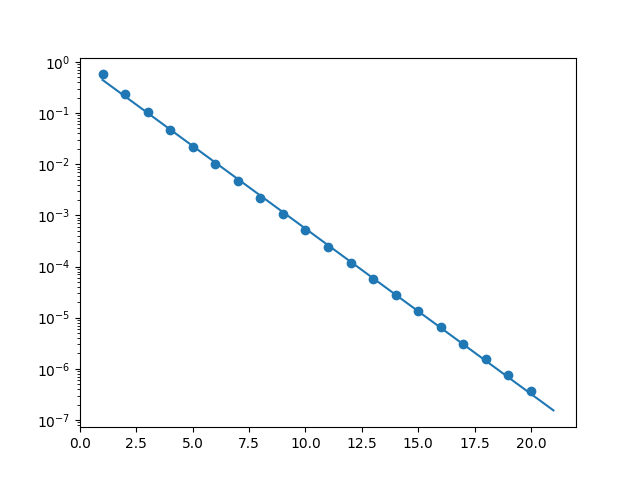
\includegraphics[width=0.8\textwidth]{3.1.6_fig.png}
\end{center}
\end{solution}


\begin{problem}{3.2.4}
Prove that if $\vec{A}$ is an invertible square matrix then $\vec{A}^+ = \vec{A}^{-1}$.
\end{problem}
\begin{solution}
\begin{align*}
    \vec{A}^+\vec{A} &= ((\vec{A}^T\vec{A})^{-1}\vec{A}^T)\vec{A} \\
    &= (\vec{A}^T\vec{A})^{-1}(\vec{A}^T\vec{A}) \\
    &= \vec{I} \\
    \vec{A}\vec{A}^+ &= \vec{A}((\vec{A}^T\vec{A})^{-1}\vec{A}^T) \\
    &= \vec{A}(\vec{A}^{-1}\vec{A}^{-T}\vec{A}^T) \\
    &= (\vec{A}\vec{A}^{-1})(\vec{A}^{-T}\vec{A}^T) \\
    &= \vec{I}    
\end{align*}
\end{solution}



\begin{problem}{3.2.5}
\begin{enumerate}[(a)]
    \item Show that for any $m \times n$ $\vec{A}$ with $m > n$ for which $\vec{A}^T\vec{A}$ is nonsingular, $\vec{A}^+\vec{A}$ is the $n \times n$ identity.
    \item Show using a computer that $\vec{A}\vec{A}^+$ is not an identity matrix. (This matrix has rank no greater than $n$, so it can't be an $m \times m$ identity.)
\end{enumerate}
\end{problem}
\begin{solution}
\begin{enumerate}[(a)]
    \item We already know that $\vec{A}^+\vec{A}$ is an identity matrix from the previous question. We just need to verify that $\vec{A}^+\vec{A}$ has size $n \times n$. To that end: $\vec{A}^+\vec{A} = ((\vec{A}^T\vec{A})^{-1}\vec{A}^T)\vec{A}$ which has size:
    \begin{align*}
        &((m \times n)^T(m \times n))^{-1}(m \times n)^T(m\times n) \\
        &= (n \times m)(m \times n)(n \times m)(m\times n) \\
        &= n \times n
    \end{align*}
    \item We just need to find an example where $\vec{A}\vec{A}^+$ is full rank. To that end, we will try a random matrix:
\begin{lstlisting}[frame=tlrb]
import numpy as np

m = 6
n = 3
A = np.random.rand(m, n)
A_pinv = np.linalg.pinv(A)
print(A @ A_pinv)
print(A_pinv @ A)
\end{lstlisting}
Output:
\begin{verbatim}
[[ 1.00000000e+00 -5.68572817e-17  7.40633706e-17]
 [ 3.59927171e-16  1.00000000e+00 -2.54025998e-16]
 [ 3.90894929e-16 -2.27010374e-16  1.00000000e+00]]
[[ 0.43538872  0.38185161  0.20938718  0.10300637 -0.10999644 -0.18292678]
 [ 0.38185161  0.39951213  0.15465099  0.26165264  0.02322982 -0.0342473 ]
 [ 0.20938718  0.15465099  0.11370954 -0.02699179 -0.10843711 -0.143292  ]
 [ 0.10300637  0.26165264 -0.02699179  0.4996222   0.1740401   0.37404402]
 [-0.10999644  0.02322982 -0.10843711  0.1740401   0.90310144 -0.18116794]
 [-0.18292678 -0.0342473  -0.143292    0.37404402 -0.18116794  0.64866596]]
\end{verbatim}
I encourage you to run this code for yourself a few times to watch what happens.
\end{enumerate}
\end{solution}


\begin{problem}{3.3.3}
Let $t_0, \ldots t_m$ be $m + 1$ equally spaced points in $[-1, 1]$. Let $\vec{A}$ be the matrix in \href{https://fncbook.com/fitting#vandersystemrect}{(3.1.2)} for $m = 400$ and fitting by polynomials of degree less than $5$. Find the thin QR factorization of $\vec{A}$, and, on a single graph, plot every column of $\hat{\vec{Q}}$ as a function of the vector $t$.
\end{problem}
\begin{solution}
The following code produces the desired decomposition of a Vandermonde matrix. (Note: in example 3.1.2, the matrix has columns corresponding to decreasing degree while this has columns corresponding to increasing degree. The result should still be the same, however.)
\begin{lstlisting}[frame=tlrb]
import numpy as np
import matplotlib.pyplot as plt

def vander(x, p):
    return np.array([[x_i**j for j in range(p)] for x_i in x])


m = 400
t = np.linspace(-1, 1, m+1)
p = 5 # degree p-1 is the approximation we are using

A = vander(t, p)
print(A)

Q, R = np.linalg.qr(A)
print(Q)

for i in range(p):
    plt.plot(t, Q[:,i], label='x^' + str(i))
plt.title('Q for a Vandermonde Matrix')
plt.xlabel('t')
plt.legend()
plt.show()
\end{lstlisting}
Output:
\begin{center}
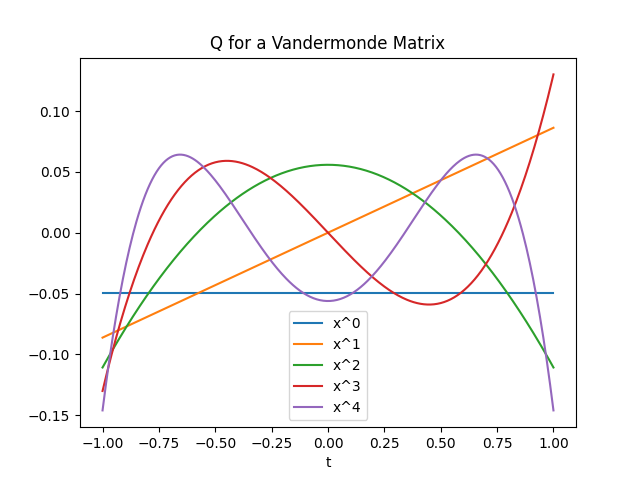
\includegraphics[width=0.8\textwidth]{3.3.3_fig.png}
\end{center}
\end{solution}


\end{document}
